% 曲线坐标系中的重积分
% 多元微积分|积分|重积分|曲线坐标系|正交曲线坐标系|极坐标系|面积法|体积分

\pentry{重积分\upref{IntN}, 正交曲线坐标系\upref{CurCor}}
在计算一些多重积分时, 选取合适的坐标系往往可以大大化简问题.

\subsection{极坐标系中的二重积分}
 
\begin{figure}[ht]
\centering
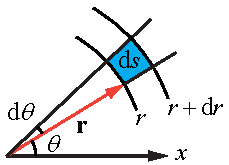
\includegraphics[width=4cm]{./figures/CrIntN_1.pdf}
\caption{极坐标中的面积元} \label{CrIntN_fig1}
\end{figure}

我们来看如何在极坐标系中进行二重积分. 我们先把积分区域划分为无数个小面元, 点 $\bvec r$ 处面元的形状如\autoref{CrIntN_fig1} 所示, 即把两个坐标 $r, \theta$ 坐标分别在原来的基础上增加一个微小值,并围成一块小区域. 由于 $\dd{r}, \dd{\theta}$ 都是无穷小, 该面元的形状趋近于长方形, 其面积为两边长相乘
\begin{equation}
\dd{s} = \dd{r}\cdot r\dd{\theta} = r\dd{r}\dd{\theta}
\end{equation}
类比\autoref{IntN_ex1}~\upref{IntN}, 我们可以将 $f(r, \theta)$ 的面积分记为
\begin{equation}\label{CrIntN_eq2}
\iint_{\mathcal S} f(r, \theta) r\dd{r}\dd{\theta} = \int_{\theta_1}^{\theta_2} \dd{\theta}\int_{r_1(\theta)}^{r_2(\theta)} \dd{r} r f(r, \theta)
\end{equation}
其中 $r_1(\theta)$ 与 $r_2(\theta)$ 是区域 $\mathcal S$ 的两条边界(类比\autoref{IntN_eq7} 中的 $y_1(x), y_2(x)$)

\begin{example}{}
求 $f(r,\theta) = ar$ 在内外半径为 $R_1, R_2$ 的圆环区域的面积分. 

先来看积分上下限, 对于圆环区域, 显然有 $r_1(\theta) = R_1$, $r_2(\theta) = R_2$, $\theta_1 = 0$, $\theta_2 = 2\pi$. 直接使用\autoref{CrIntN_eq2} 得
\begin{equation}\ali{
\iint_{\mathcal S} f(r, \theta) r\dd{r}\dd{\theta} &= \int_0^{2\pi} \qty[\int_{R_1}^{R_2} ar^2 \dd{r}] \dd{\theta}
= \int_0^{2\pi} \frac a3 (R_2^3 - R_1^3) \dd{\theta}\\
&= \frac{2\pi a}{3} (R_2^3 - R_1^3)
}\end{equation}

如果使用直角坐标系计算该积分, 过程将会变得十分复杂.
\end{example}

\subsection{曲线坐标系中的体积分}
在曲线坐标系中, 令
\begin{equation}\label{CrIntN_eq7}
\pdv{\bvec r}{x_i} \equiv f_i(\bvec r)\uvec x_i \quad (i = 1,2,3)
\end{equation}
则位矢的全微分为
\begin{equation}\label{CrIntN_eq8}
\dd{\bvec r} = \sum_{i = 1}^3 f_i(\bvec r)\dd{x_i}\uvec x_i
\end{equation}
所以空间中的一个体积元(每个 $x_i$ 都分别增加 $\dd{x_i}$ 所围成的长方体)可以表示为
\begin{equation}
\dd{V} = f_1(\bvec r)f_2(\bvec r)f_3(\bvec r)\dd{x_1}\dd{x_2}\dd{x_3}
\end{equation}
这是因为根据\autoref{CrIntN_eq8}, 单独将坐标 $x_i$ 增加 $\dd{x_i}$ 会导致 $\bvec r$ 在 $\uvec x_i$ 方向增加 $f_i(\bvec r)\dd{x_i}$, 这相当于长方体在 $\uvec x_i$ 方向的边长, 而长方体的体积等于三条边长之积. 为了方便书写我们以后将 $\dd{x_1}\dd{x_2}\dd{x_3}$ 记为 $\dd[3]{x}$ 或 $\dd[3]{r}$.
\begin{figure}[ht]
\centering
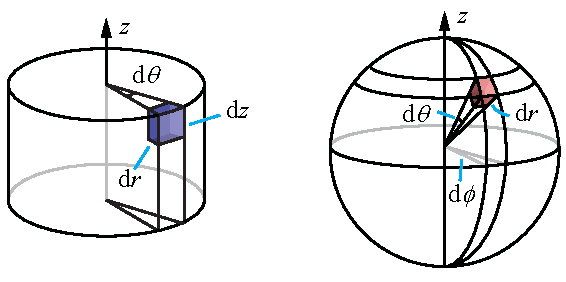
\includegraphics[width=9.5cm]{./figures/CrIntN_2.pdf}
\caption{柱坐标(左)和球坐标(右)中的体积元} \label{CrIntN_fig2}
\end{figure}

我们已知直角坐标系中 $\pdv*{\bvec r}{x_i} = 1$, 所以体积元为 $\dd[3]{r} = \dd{x}\dd{y}\dd{z}$. 对于柱坐标系(\autoref{CrIntN_fig2} 左), 由\autoref{CurCor_eq5}~\upref{CurCor} 得体积元为
\begin{equation}
\dd{V} = \dd{r}\cdot r\dd{\theta} \cdot \dd{z} = r\dd{r}\dd{\theta}\dd{z}
\end{equation}
类似地, 对于球坐标系(\autoref{CrIntN_fig2} 右), 由\autoref{CurCor_eq11}~\upref{CurCor} 得体积元为
\begin{equation}
\dd{V} = \dd{r} \cdot r\dd{\theta} \cdot r\sin\theta\dd{\phi} = r^2\sin\theta\dd{r}\dd{\theta}\dd{\phi}
\end{equation}

\begin{example}{球体的体积}
在\autoref{DefInt_ex4}~\upref{DefInt} 中我们用一元函数的定积分得到了球体的体积, 现在我们也可以直接在球坐标中由体积分得到.
\begin{equation}\ali{
V &= \int 1 \dd[3]{r} = \int_0^{2\pi} \int_0^\pi \int_0^R   r^2\sin\theta \dd{r} \dd{\theta} \dd{\phi}\\
&= \int_0^{2\pi} \dd{\phi} \int_0^\pi \sin\theta \dd{\theta} \int_0^R   r^2 \dd{r}\\
&= 2\pi \cdot 2 \cdot \frac 13 R^3 = \frac 43 \pi R^3
}\end{equation}
\end{example}